%----------------------------------------------------
% Setup Beamer
%----------------------------------------------------
\documentclass[hyperref={colorlinks=true}]{beamer}

%----------------------------------------------------
% Packages to use
%----------------------------------------------------
\input{../packages.sty}

%----------------------------------------------------
% Setup Theme
%----------------------------------------------------
\input{../theme.sty}

%----------------------------------------------------
% Table of Contents at each section transition
%----------------------------------------------------

\AtBeginSection[]
{
   \begin{frame}
       \frametitle{Outline}
       \setcounter{tocdepth}{2}
       \tableofcontents[currentsection]
   \end{frame}
}

%----------------------------------------------------
% Colors
%----------------------------------------------------
\input{../mycolors.sty}

%----------------------------------------------------
% Style, formatting, and new commands
%----------------------------------------------------
\newcommand{\CourseYear}   {2024}
\newcommand{\CanvasURL}    {https://canvas.uchicago.edu/courses/58627}
\newcommand{\CanvasLink}   {\href{\CanvasURL}{\CanvasURL}}
\newcommand{\GitHubURL}    {https://github.com/UChicagoPhysics/PHYS250}
\newcommand{\GitHubLink}   {\href{\GitHubURL}{\GitHubURL}}
\newcommand{\PlatformURL}  {https://binderhub.pile.uchicago.edu/}
\newcommand{\PlatformLink} {\href{\PlatformURL}{\PlatformURL}}
\newcommand{\PiazzaURL}    {https://canvas.uchicago.edu/courses/58627/discussion\_topics}
\newcommand{\PiazzaLink}   {\href{\PiazzaURL}{\PiazzaURL}}
\input{../newcommands.sty}
\input{../EandMcommands.sty}

%----------------------------------------------------
% Set paths for plots and images
%----------------------------------------------------
\input{../paths.sty}


%-----------------------------------------------------------------------------------------
% Title: [Column]{Title}
%-----------------------------------------------------------------------------------------
\title[PHYS 250 (Autumn 2024) -- Lecture 6]{Ising model (cont'd)}

%-----------------------------------------------------------------------------------------
% SubTitle: [Column]{Subtitle}
%-----------------------------------------------------------------------------------------
\subtitle{PHYS 250 (Autumn 2024) -- Lecture 6}

%-----------------------------------------------------------------------------------------
% Author: [SubAuthor]{Author}
%-----------------------------------------------------------------------------------------
\author[D.W.~Miller]{David Miller}

%----------------------------------------------------
% Institute: [SubInst]{Institute}
%----------------------------------------------------
\institute[EFI, Chicago] 
{
  Department of Physics and the Enrico Fermi Institute\\
  University of Chicago
}

%----------------------------------------------------
% Institute: [SubInst]{Institute}
%----------------------------------------------------
\date[October 17, 2024]{October 17, 2024}

\subject{PHYS 250 Lecture}

\begin{document}

%==========================================================================================
% TITLE PAGE
%==========================================================================================

{
\begin{frame}
  \titlepage
\end{frame}
}

%==========================================================================================
\section[Computational Ising model]{Computational Ising model}
%==========================================================================================

%-----------------------------------------------------------------------------------------
\subsection[Reminders]{Reminders}
\begin{frame}%[shrink=10]
  \frametitle{Quantum mechanics of the Ising model}

  \begin{columns}
  
  \column{0.5\textwidth}
  
  The Hamiltonian for a system of $N$ spins $s_i$ in free space, which may take on values of $s_i = \pm1$ is given by the interaction of the spins
  %
  \begin{equation}
    \Ham = -J \sum_{\mean{ij}}^N s_i s_{j} , \label{eq:ising-free}
  \end{equation} 
  %
  where the sum \mean{ij} is over all pairs of nearest-neighbor sites, $J$ is the \alertbf{coupling} between these neighboring sites. (For example, there are four neighbors per site on the square lattice.)
  
  \vspace{-0.5cm}
  
    \begin{figure}
      \centering
      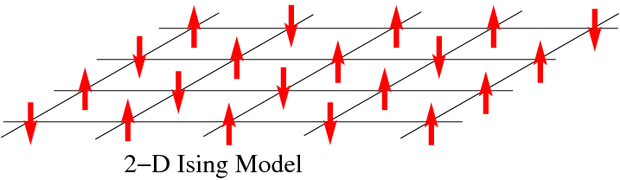
\includegraphics[width=0.8\columnwidth]{Ising-spins-2D.png}
    \end{figure}
    
  \column{0.45\textwidth}
  
    \begin{figure}
      \centering
      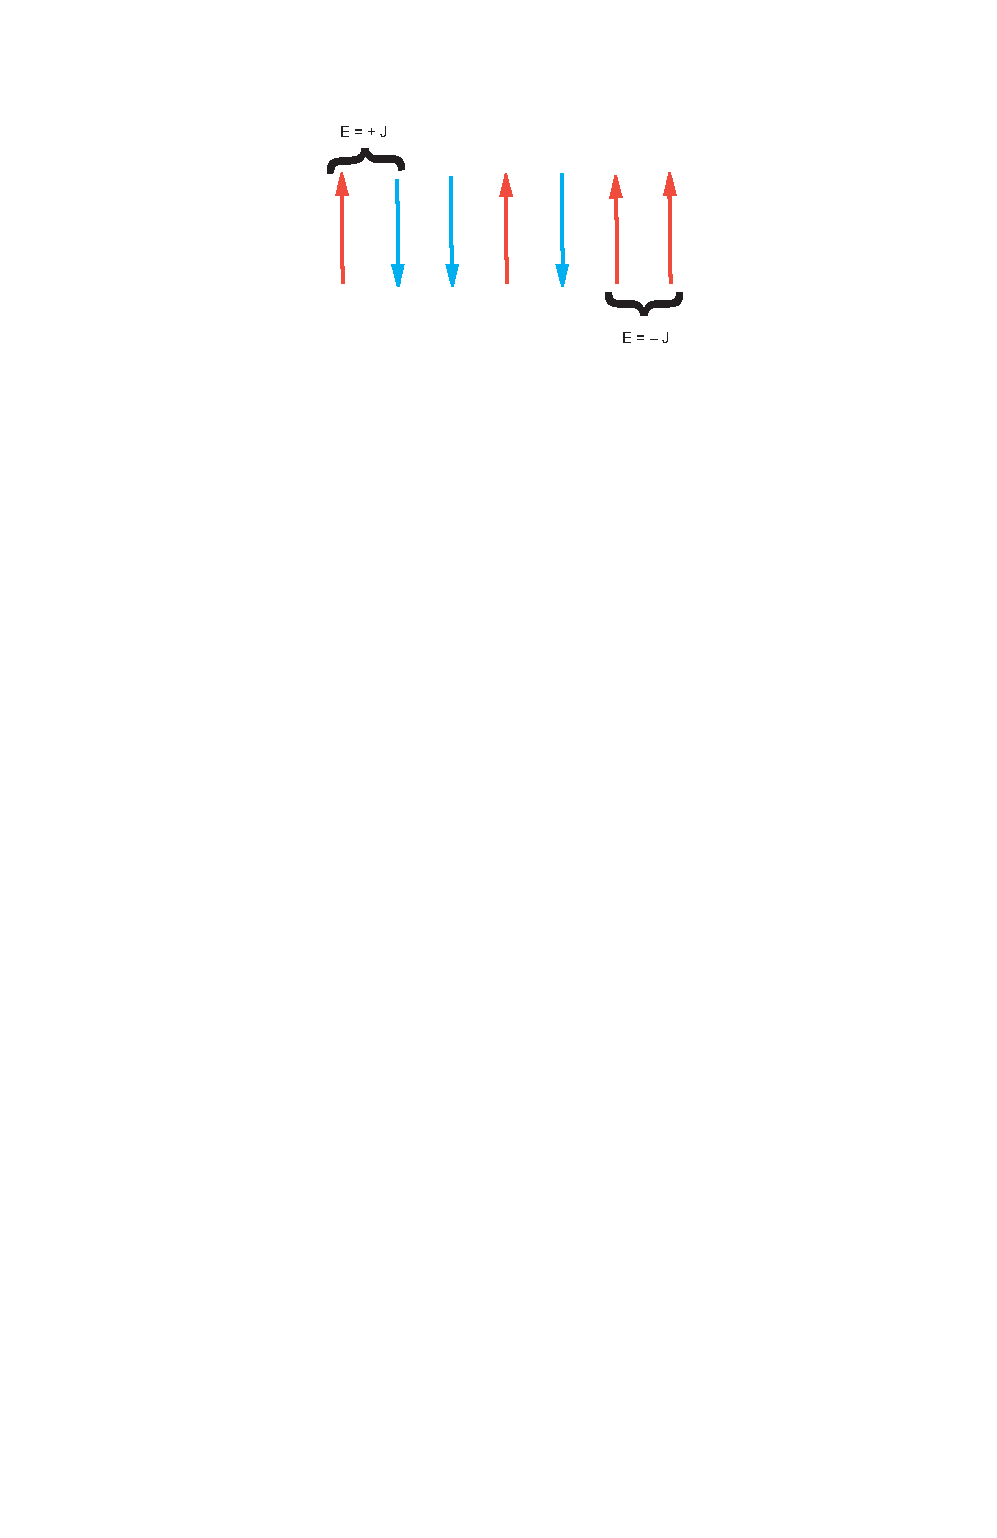
\includegraphics[width=\columnwidth]{Ising-spins-1D-interaction.pdf}\\
      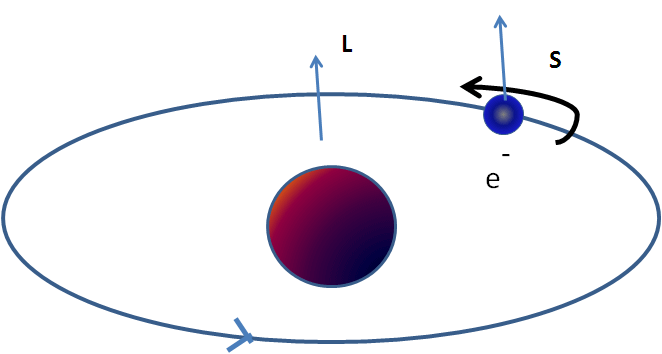
\includegraphics[width=\columnwidth]{SpinOrbitMoment.png}
    \end{figure}
  
  \end{columns}

  

\end{frame}

%-----------------------------------------------------------------------------------------

\begin{frame}%[shrink=10]
  \frametitle{Magnetism and spins (I)}

  As we've discussed in E\&M, magnetism is caused by charged particles \bluebf{``spinning''} in closed orbits or about their axes
  %
  \begin{itemize}
    \item For elementary particles, of course, we mean ``spinning'' in the quantum mechanical sense, not the rotational Newtonian sense
  \end{itemize}
  %
  So atoms may have \bluebf{both an $L$ (orbit) and an $S$ (spin) contribution} (capital letters for ``operators'' for those of you in the know) to the magnetic properties. For the Ising model, we're concerned with just a single contribution which we will refer to as $s$ as on the previous slide.
  
  \vspace{0.3cm}
  
  In addition to the contribution to the Hamiltonian (and thus the energy) from the spin-spin interactions, there is the possibility that we apply an external magnetic field, $H$:
  %
  \begin{equation}
    \Ham = -J \sum_{\mean{ij}}^N s_i s_{j} - H \sum_i s_i , \label{eq:ising-field}
  \end{equation} 

  Note that the ``magnetization'' is given by $M=\sum_i s_i$.

\end{frame}



%-----------------------------------------------------------------------------------------

\begin{frame}%[shrink=10]
  \frametitle{Magnetism and spins (II)}

  Let's discuss our Hamiltonian
  %
  \begin{equation}
    \Ham = -J \sum_{\mean{ij}}^N s_i s_{j} - H \sum_i s_i , \label{eq:ising-field}
  \end{equation} 
  %
  \begin{itemize}
    \item \bluebf{If $J > 0$ : ferromagnetic}
    \begin{itemize}
      \item Energy is minimized if the spins point in the same direction
    \end{itemize}
    \item \bluebf{If $J < 0$ : antiferromagnetic}
    \begin{itemize}
      \item Energy is minimized if spins locally point in the opposite direction
    \end{itemize}
  \end{itemize}
  
  \begin{ucblock}{Important observations which we will study}
    \begin{itemize}
      \item At low temperatures, the \bluebf{spins will organize themselves} to either mostly point up or mostly point down, forming a ferromagnetic phase.
      \item The spins will tend to align (in a 2D square lattice) in a \bluebf{checkerboard antiferromagnetic phase} at low temperatures. 
      \item At high temperatures, independent of the sign of $J$, we expect entropy to dominate; the spins will fluctuate wildly in a \bluebf{paramagnetic phase} and the magnetization per spin $m(T ) = M (T )/N$ is zero 
    \end{itemize}
  \end{ucblock}
    
\end{frame}

%-----------------------------------------------------------------------------------------

\begin{frame}%[shrink=10]
  \frametitle{Emergent properties of the Ising model}
  
    \begin{figure}
      \centering
      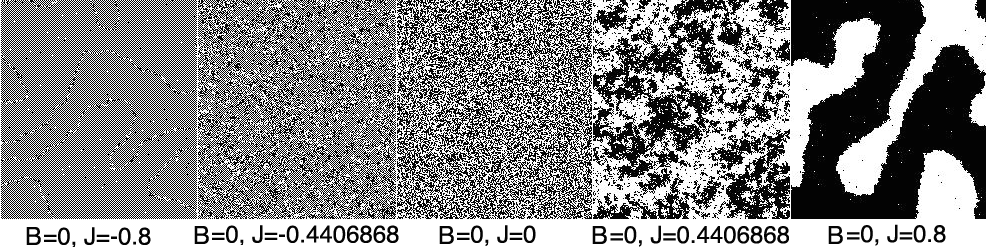
\includegraphics[width=\columnwidth]{IsingDomains.png}
    \end{figure}
  
  Amazing features result from the \bluebf{ensemble behavior} of the lattice sites of a 2D Ising model. Phase transitions, criticality, and other phenomena are all part of what we will study computationally with this model. 

  \begin{figure}
      \centering
      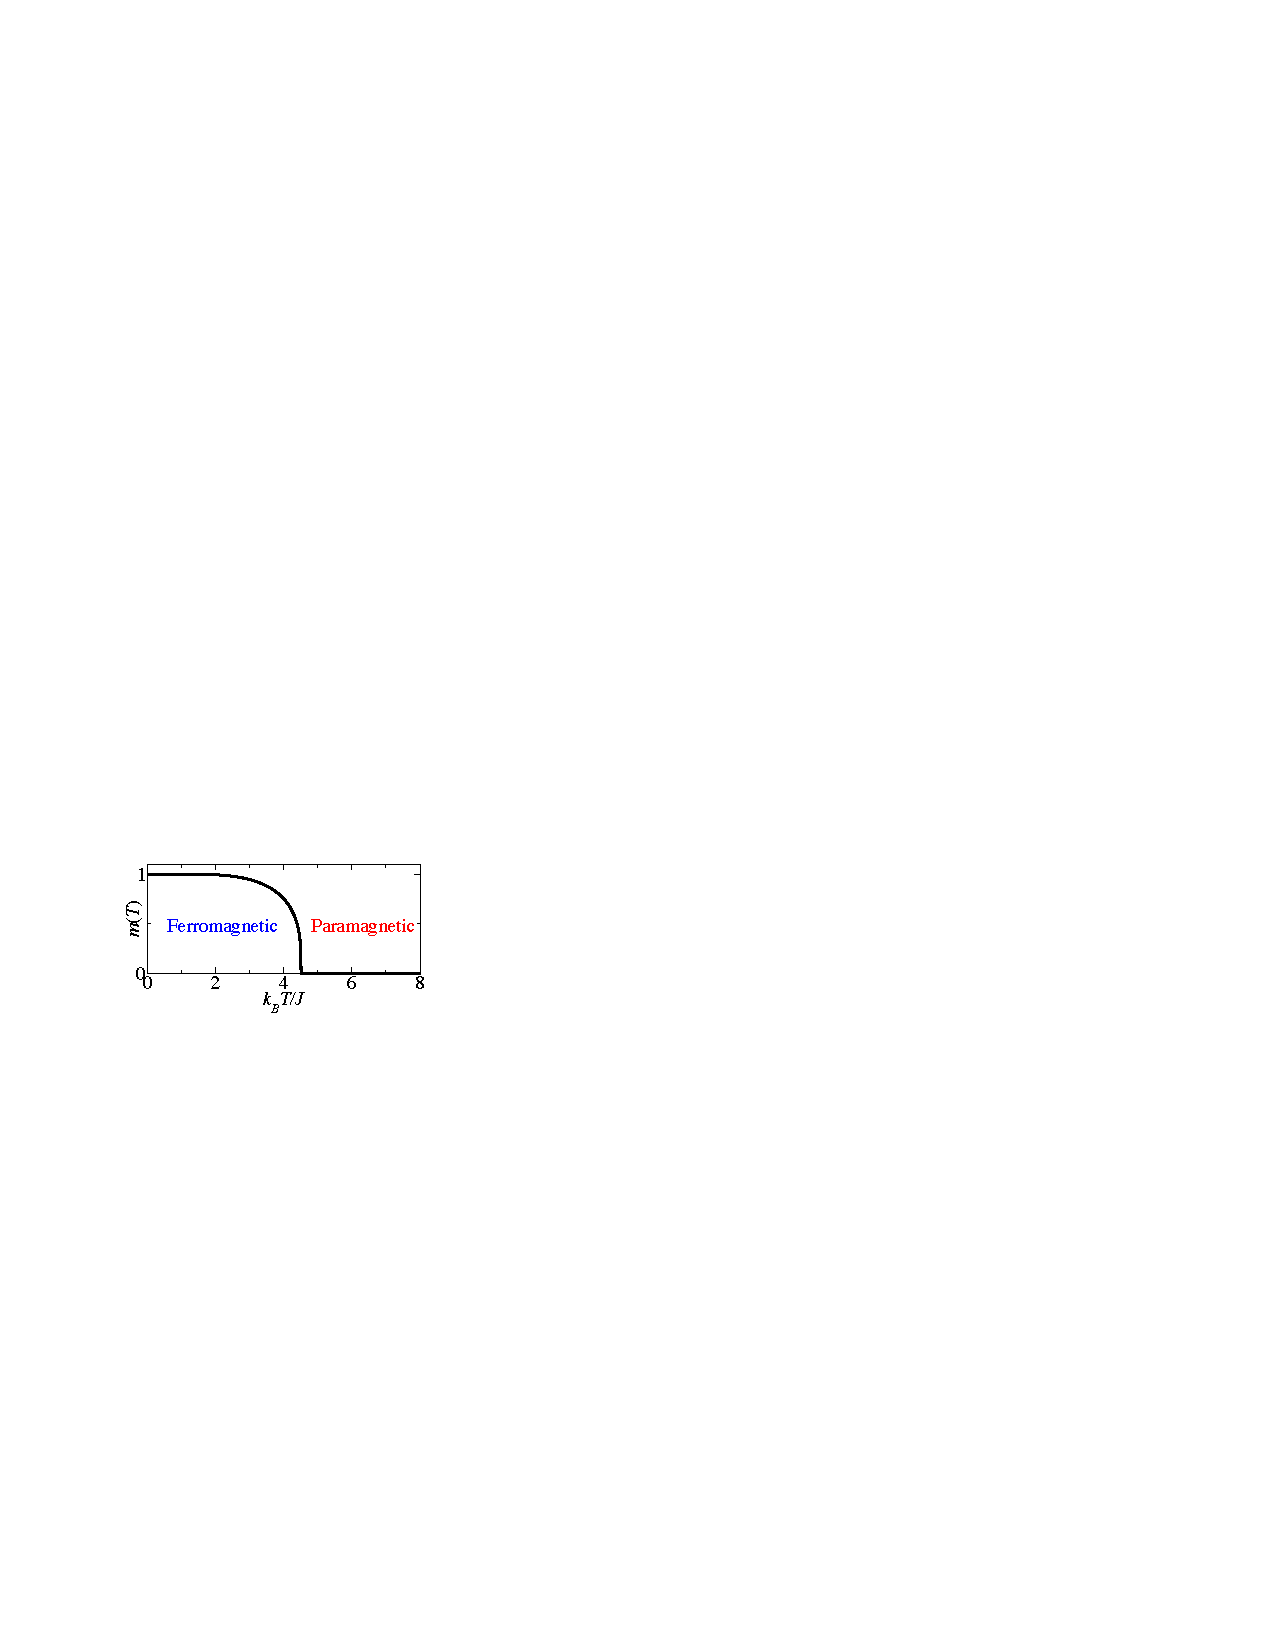
\includegraphics[width=0.5\columnwidth]{MagnetizationPerSpin.pdf}
  \end{figure}
  
\end{frame}


%-----------------------------------------------------------------------------------------

\begin{frame}%[shrink=10]
  \frametitle{A few quantum mechanics notes}
  
  The Ising model parameters are rescaled from the microscopic ones. The Ising spin $s_i = \pm1$ represents twice the $z$-component of a spin-1/2 atom in a crystal, $\sigma_i^z = s_i/2$. 
  
  \vspace{0.5cm}
  
  The Ising interactions between spins, $J s_i s_j = 4 J \sigma_i^z \sigma_j^z$, is thus shifted by a factor of four from the $z-z$ coupling between spins. 
  
  \vspace{0.5cm}
  
  The coupling of the spin to the external magnetic field is microscopically $g \mu_B H \cdot \sigma_i^z$, where $g$ is the gyromagnetic ratio for the spin (close to two for the electron) and $\mu_B = \frac{e \hbar}{2 m_e}$ is the Bohr magneton. 
  
  \vspace{0.5cm}
  
  \bluebf{Hence, for those of you who've taken quantum mechanics, the Ising external field is rescaled from the physical one by $g \mu_B / 2$. }

\end{frame}



%-----------------------------------------------------------------------------------------
\subsection[Practical implications and relationships]{Practical implications and relationships}
%-----------------------------------------------------------------------------------------

\begin{frame}%[shrink=10]
  \frametitle{Broader context for the Ising model}
  
  Lattice models are a big industry within statistical mechanics. Many systems and their computational evaluation and study take place on a lattice:
  
  \begin{itemize}
    \item \bluebf{Critical phenomena and phase transitions}
    \item \bluebf{lattice QCD and quantum field theories}
    \item \bluebf{quantum magnetism and models for high-temperature superconductors}
    \item \bluebf{phase diagrams for alloys}
    \item \bluebf{the behavior of systems with dirt or disorder}
    \item \bluebf{non-equilibrium systems exhibiting avalanches and crackling noise}
  \end{itemize}
  
  And many more!
  
  \center \textit{(now do you see why I spent time showing you \texttt{np.mgrid}?!)}
  
\end{frame}

%-----------------------------------------------------------------------------------------
\subsection[Complications and numerical and computational obstacles]{Complications and numerical and computational obstacles}
%-----------------------------------------------------------------------------------------

%-----------------------------------------------------------------------------------------

\begin{frame}%[shrink=10]
  \frametitle{Computational complexity and simulation}
  
  The 1D model was solved analytically in 1924. 
  
  \vspace{0.3cm}
  
  The 2D model was not solved analytically until Lars Onsager did it in 1944. 
  \begin{itemize}
    \item Onsager solved is using the \bluebf{ transfer-matrix method}, where you essentially break up the partition function, $Z$ into many pieces and decompose the interactions in a matrix formulation and then do an eigenvector decomposition and solve it that way. 
  \end{itemize}
  
  \vspace{0.3cm}
  
  However, this only really works for a small system. If there are many states (i.e. many sites) it can easily become analytically intractable even if solvable in principle.
  
  \vspace{0.3cm}
  
  \begin{ucblock}{}
     \textbf{Instead, we will approach this using our Monte Carlo based approach!}
  \end{ucblock}
   
\end{frame}

%-----------------------------------------------------------------------------------------

\begin{frame}%[shrink=10]
  \frametitle{Reminder of the Ising model}
  
  In \href{https://github.com/UChicagoPhysics/PHYS250/blob/master/Slides/Lecture5/PHYS250-Fall2019-Lecture5.pdf}{Lecture 5} we began discussing the Ising model and the general principles that we seek to understand about this deceptively \alertbf{``simple''} model for a set of spin states $\spins = \{\spini\}$, with a Hamiltonian, \Ham, for a given interaction coupling, $J$, and magnetic field, $H$, given by:
  
  \begin{equation}
    \Ham = -J \sum_{\mean{ij}}^N \spini \spinj - H \sum_i \spini , \label{eq:ising-field}
  \end{equation} 
  
  \begin{ucblock}{}
    \bluebf{Given a randomized set of $N$ spins, the Ising model has $2^N$ states $\spins = \{\spini\}$ in $d=2$ dimensions. What happens to the system when we let it evolve according to the laws of statistical mechanics? Does the average spin remain random? How does the application of an external field affect its evolution? Can we calculate a specific heat for this system (the temperature change required to raise the system's energy by a given amount)?} 
  \end{ucblock}
  
\end{frame}

%-----------------------------------------------------------------------------------------

\begin{frame}%[shrink=10]
  \frametitle{The statistical mechanics of the system}
  
  The energy $E_{\mu}$ of a particular microstate $\mu$ of this (discrete) system is given by the operator \Ham acting on that microstate, or specific  $\spins = \spinsmu$. We assume that although the system is in an \bluebf{equilibrium state} (i.e. the energy of a particular element is proportional to the temperature, $T$), it is a dynamic one in which each element's energy fluctuates as it exchanges energy with its environment. The probability for the ensemble \spins to have energy $E_{\mu}$ is 
  
  \begin{equation}
    P(\spinsmu) = \frac{e^{-\beta E_{\mu}}}{\sum_{\mu} e^{-\beta E_{\mu}}},
  \end{equation} 

  And the mean and variance of the energy $\mean{E}$ (or \textit{any} observable) is given by 
  
  \begin{eqnarray}
    \mean{E} &=& \sum_{\mu} E_{\mu} P(\spinsmu) = \frac{1}{Z} \sum_{\mu} E_{\mu} e^{-\beta E_{\mu}} \\
    Var(E) = \mean{(E-\mean{E}^2)^2} &=& \sum_{\mu} E^2_{\mu} P(\spinsmu) - \left( \sum_{\mu} E_{\mu} P(\spinsmu) \right)^2
  \end{eqnarray} 
  
\end{frame}

%-----------------------------------------------------------------------------------------

\begin{frame}%[shrink=10]
  \frametitle{Computational obstacles (big ones)}
  
  If we were to brute-force calculate the sum in the previous slide, we would have to perform $4 \times N \times 2^{N}$ calculations, which quickly becomes $\sim\infty$. For example, for just a $5\times 5$ lattice, we have $2^{25} = 33,554,432$ states. For a $100\times100$ lattice, well...
  
  \pause
  
  \begin{figure}
    \centering
    \includegraphics<2>[width=0.75\columnwidth]{Calculator.jpg}
  \end{figure}
  
  \pause
    
  We can save summing over half of these due to up/down symmetry, which means that for every state there is another one in which every spin is simply flipped upside down, with exactly the same energy (for $H=0$). So, we can simplify the calculation by just taking one out of every pair of such states, for a total of $16,777,216$ states, and summing up the corresponding terms in the partition function.
  
  \vspace{0.3cm}
  
  We could save further time by using other symmetries too. For example, a square lattice also has a reflection symmetry and a four-fold rotational symmetry (symmetry group $C_4$), meaning that the states actually group into sets of 16 states (including the up/down symmetry pairs), all of which have the same energy. But $\infty/16$ still ain't great...
  
\end{frame}

%-----------------------------------------------------------------------------------------
\subsection[Monte Carlo Methods]{Monte Carlo Methods}
%-----------------------------------------------------------------------------------------

\begin{frame}%[shrink=10]
  \frametitle{Monte Carlo methods}
  
  There is essentially only \alertbf{one known numerical method} for calculating the partition function of a model such as the Ising model on a large lattice, and that method is \bluebf{Monte Carlo simulation}. 
  
  \begin{itemize}
    \item If we are clever enough, we can obtain a \bluebf{relatively good estimate} by only performing a \alertbf{subset} of the calculations, $\{\mu\}$ instead of all $\mu$
    \item One way to be clever is to only sample the distribution that we are attempting to model, $P(\spinsmu)$ in regions where it is important.
    \item To put it another way, we want to perform a \alertbf{weighted sampling}
  \end{itemize}
  %
  \begin{eqnarray}
    \mean{E} &=& \frac{\sum_{\{\mu\}} E_{\mu} e^{-\beta E_{\mu}} W_{\mu}^{-1}}{\sum_{\{\mu\}} e^{-\beta E_{\mu}} W_{\mu}^{-1}} \\
       &\approx& \frac{\sum_{\{\mu\}} E_{\mu}}{\sum_{\{\mu\}} 1} = \frac{1}{N^{\prime}}\sum_{\{\mu\}} E_{\mu}
  \end{eqnarray} 
  %
  where $N^{\prime}$ is the number of terms in the subset $\{\mu\}$ and $W_{\mu} = e^{- \beta E_{\mu}}/Z$.
  
\end{frame}

%-----------------------------------------------------------------------------------------

\begin{frame}%[shrink=10]
  \frametitle{Recap of the Monte Carlo methods}

   We discussed (briefly) two approaches to the Monte Carlo implementation
   
   \begin{itemize}
     \item \bluebf{Heat bath method:} always flip a spin according to the Boltzmann factor based on the energy difference (i.e. an energy difference of $\Delta E = 0$ has a 50\% probability of flipping)
     \item \bluebf{Metropolis method:} always flip a spin if the energy difference is negative (i.e. the new spin configuration results in a lower energy), but only flip the spin according to the Boltzmann factor if the result is an energy increase.
   \end{itemize}
 
   In both cases, there are two underlying assumptions which were first proposed in 1949 by Nicolas Metropolis (hence the eponymous algorithm).
 
\end{frame}

%-----------------------------------------------------------------------------------------
\subsection[The origins of Monte Carlo]{The origins of Monte Carlo}
%-----------------------------------------------------------------------------------------

\begin{frame}%[shrink=10]
  \frametitle{The beginning of the Monte Carlo}
  
  The idea of Monte Carlo calculation is a lot older than the computer. Under the older name of ``statistical sampling'' the method has a history stretching back well into the last century, when numerical calculations were performed by hand using pencil and paper and perhaps a slide-rule.
  
  \vspace{0.3cm}
  
  \bluebf{The name ``Monte Carlo'' is relatively recent:} it was \href{https://www.tandfonline.com/doi/abs/10.1080/01621459.1949.10483310}{coined by Nicolas Metropolis in 1949 in a paper with Stanislav Ulam}
  
  \begin{figure}
    \centering
    \frame{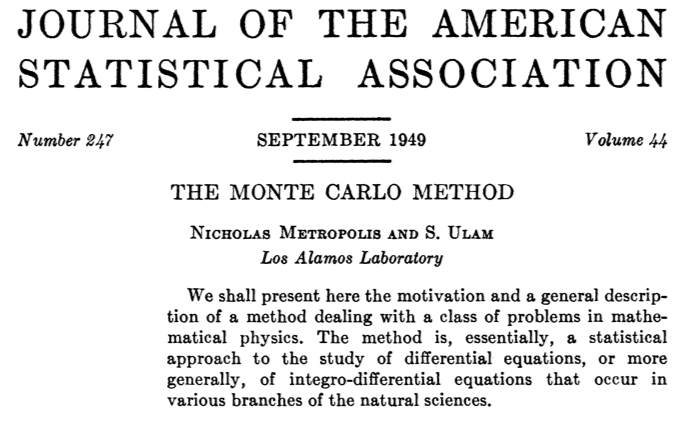
\includegraphics[width=0.65\columnwidth]{MonteCarlo.pdf}}
  \end{figure}
  
\end{frame}

%-----------------------------------------------------------------------------------------

\begin{frame}[shrink=20]
  \frametitle{Nicolas Metropolis}
  
  Nicholas Constantine Metropolis was born in 1915, in Chicago (where all the coolest people were born). In 1936 he received his bachelor's degree, and in 1941, his doctorate, both from UChicago, and both in experimental physics. While here, Metropolis worked at the Met Lab as an assistant to Fermi. The MANIAC was Metropolis' computer at Los Alamos:  \bluebf{``Mathematical Analyzer, Numerical Integrator, and Computer''}. In 1957, Metropolis returned to UChicago and founded the Institute for Computer Research. Here, he oversaw the construction MANIACIII machine.
  
  \vspace{-0.4cm}
  
  \begin{columns}
  
    \column{0.5\textwidth}
    
      \begin{figure}
        \centering
        \includegraphics[width=0.7\columnwidth]{MANIACII.jpg}\\
        \includegraphics[width=0.7\columnwidth]{MANIACIII.jpg}
      \end{figure}
    
    \column{0.5\textwidth}
    
      \begin{figure}
        \centering
        \includegraphics[width=0.8\columnwidth]{FermiPhaseShiftComputation.pdf}
      \end{figure}
  
  \end{columns}
  
\end{frame}



%-----------------------------------------------------------------------------------------

\begin{frame}%[shrink=10]
  \frametitle{The concepts behind Monte Carlo}
  
  The concept that Metropolis and Ulam sketched out is exactly what we have been discussing:
  
  \begin{figure}
    \centering
    \frame{\includegraphics[width=0.95\columnwidth]{MonteCarloConcept.pdf}}
  \end{figure}
  
  but is also has a very important embedded concept from deep within statistical physics (we will come back to this in a moment):
  
  \begin{figure}
    \centering
    \frame{\includegraphics[width=\columnwidth]{Ergodic.pdf}}
  \end{figure}
  
\end{frame}

%-----------------------------------------------------------------------------------------

\begin{frame}%[shrink=10]
  \frametitle{Computational physics was born}
  
  In the same paper, Metropolis and Ulam made a compelling suggestion: with a combination of good ideas (from Fermi) and computers, this could be very powerful!
  
  \begin{figure}
    \centering
    \frame{\includegraphics[width=0.9\columnwidth]{ModernComputingMachines.pdf}}\\
    :\\
    \frame{\includegraphics[width=0.9\columnwidth]{FermisSuggestion.pdf}}
  \end{figure}
  
\end{frame}

%-----------------------------------------------------------------------------------------

\begin{frame}%[shrink=10]
  \frametitle{Deploying the tools}
  
  In a follow-up paper, now with some of the Manhattan project's heaviest hitters (from Chicago, of course) they put those ideas into action
  
  \begin{figure}
    \centering
    \frame{\includegraphics[width=\columnwidth]{EquationOfStateFastComputingMachines.pdf}}
  \end{figure}
  
\end{frame}

%-----------------------------------------------------------------------------------------

\begin{frame}%[shrink=10]
  \frametitle{The Metropolis algorithm}
  
  It is in this paper that the proposal to use a Boltzmann factor for attempting the \alertbf{trials} a given change in configuration
  
  \begin{center}
  \begin{minipage}{0.8\columnwidth}
  \begin{framed}
  \begin{figure}
    \centering
    \includegraphics[width=\columnwidth]{MetropolisWeight1.pdf}\\
    \includegraphics[width=\columnwidth]{MetropolisWeight2.pdf}
  \end{figure}
  \end{framed}
  \end{minipage}
  \end{center}
  
  \vspace{-0.2cm}
  
  \begin{figure}
    \centering
    \frame{\includegraphics[width=0.8\columnwidth]{ConclusionsMetropolis.pdf}}
  \end{figure}
  
\end{frame}

%-----------------------------------------------------------------------------------------
\subsection[Assumptions of the Metropolis algorithm]{Assumptions of the Metropolis algorithm}
%-----------------------------------------------------------------------------------------

\begin{frame}%[shrink=10]
  \frametitle{The Metropolis algorithm's assumptions: ergodicity}
  
  Over a sufficiently long period of time, \bluebf{all accessible microstates will be sampled}. A corollary is that the time spent by a system in some region of the phase space of microstates with the same energy is proportional to the volume of this region. 

  \vspace{0.3cm}
  
  The implication for our computational approach is that in principle, it should be \bluebf{possible for our Markov process to reach any state of the system from any other state}, if we run it for long enough. 
  
  \vspace{0.3cm}
  
  The condition of ergodicity tells us that we are allowed to make some of the transition probabilities of our Markov process zero, but that there must be at least one path of non-zero transition probabilities between any two states that we pick. 
  
  \vspace{0.3cm}
  
  In practice, most Monte Carlo algorithms set almost all of the transition probabilities to zero, and we \alertbf{must be careful that in so doing we do not create an algorithm which violates ergodicity}.

\end{frame}

%-----------------------------------------------------------------------------------------

\begin{frame}%[shrink=10]
  \frametitle{The Metropolis algorithm's assumptions: detailed balance}
  
  The detailed balance equation then tells us that the transition probabilities should satisfy
  
  \begin{equation}
    \frac{P(\mu \ra \nu)}{P(\nu \ra \mu)} = \frac{P(\spins_{\nu})}{P(\spins_{\mu})} = e^{- \beta (E_{\nu} - E_{\mu})} = e^{- \beta \Delta E}
  \end{equation}
  
  This equation and the requirement that the sum of all probabilities is unity are the basic constraints on our choice of transition probabilities. If we satisfy these, as well as the condition of ergodicity, then the equilibrium distribution of states in our Markov process will be the Boltzmann distribution. It is also useful to break this down a bit further:
  %
  \begin{eqnarray}
    P(\mu \ra \nu) &=& g(\mu \ra \nu) A(\mu \ra \nu) \\
    \frac{P(\mu \ra \nu)}{P(\nu \ra \mu)} &=& \frac{g(\mu \ra \nu) A(\mu \ra \nu)}{g(\nu \ra \mu) A(\nu \ra \mu)}
  \end{eqnarray}
  %
  where $g$ is a \bluebf{selection probability} and $A$ is the \alertbf{acceptance ratio}
\end{frame}

%-----------------------------------------------------------------------------------------

\begin{frame}%[shrink=10]
  \frametitle{Selection probability}
  
  \begin{itemize}
    \item \bluebf{$g(\mu \ra \nu)$ is the selection probability}
    \begin{itemize}
      \item this is the probability, given an initial state $\mu$, that our algorithm will generate a new target state $\nu$. 
    \end{itemize}
    \item \bluebf{$A(\mu \ra \nu)$ is the acceptance ratio (sometimes also called the ``acceptance probability'')}
    \begin{itemize}
      \item The acceptance ratio says that if we start off in a state $\mu$ and our algorithm generates a new state $\nu$ from it, we should accept that state and change our system to the new state $\nu$ a fraction of the time $A(\mu \ra \nu)$. 
      \item The rest of the time we should just stay in the state $\mu$.
      \item If the acceptance ratios for our moves are low, then the algorithm will on most time steps simply stay in the state.
    \end{itemize}
  \end{itemize}
  
  In the Metropolis algorithm the selection probabilities $g(\mu \ra \nu)$ for each of the possible states $\nu$ are all chosen to be equal.
  
\end{frame}

%-----------------------------------------------------------------------------------------

\begin{frame}%[shrink=10]
  \frametitle{Acceptance probability}
  
  \begin{figure}
    \centering
    \includegraphics[width=\columnwidth]{MetropolisAlgorithmAcceptanceRatio.pdf}
  \end{figure}
  
\end{frame}

%-----------------------------------------------------------------------------------------
%\subsection[Accept-reject algorithms]{Accept-reject algorithms}
%-----------------------------------------------------------------------------------------

%-----------------------------------------------------------------------------------------
\subsection[Metropolis-Hastings algorithm]{Metropolis-Hastings algorithm}
%-----------------------------------------------------------------------------------------
%-----------------------------------------------------------------------------------------


\begin{frame}%[shrink=10]
  \frametitle{Metropolis Monte Carlo}
  
  ``Pseudocode'' for the Metropolis algorithm:
  
  \begin{enumerate}
    \item Choose initial configuration
    \item For all spins:
    \begin{enumerate}
      \item Trial flip ($+1 \ra -1$ or vice versa)
      \item Compute change in energy
      \item If $\delta = e^{- \Delta E/\kB T} > r$ (where $r$ is a uniform deviate) flip the spin 
    \end{enumerate}
  \end{enumerate}
  
    
\end{frame}






%%==========================================================================================
%\section[Conclusions]{Conclusions}
%==========================================================================================
%
%\begin{frame}%[shrink=1]
%  \frametitle{Conclusions}
%
%  \begin{itemize}
%    \item Something
%  \end{itemize}
%  
%\end{frame}

%==========================================================================================
%==========================================================================================
\end{document}
